\documentclass{article}

\usepackage{graphicx}
\usepackage{tikz}
\usepackage{tikzsymbols}
\usetikzlibrary{calc,patterns,shapes.geometric}
\pagestyle{empty}
\usepackage[margin=0pt]{geometry}
\geometry{papersize={14in,12in}}

\def\centerarc[#1](#2)(#3:#4:#5){\draw[#1] ($(#2)+({#5*cos(#3)},{#5*sin(#3)})$) arc (#3:#4:#5);}

\begin{document}
	\begin{figure}
		\centering
		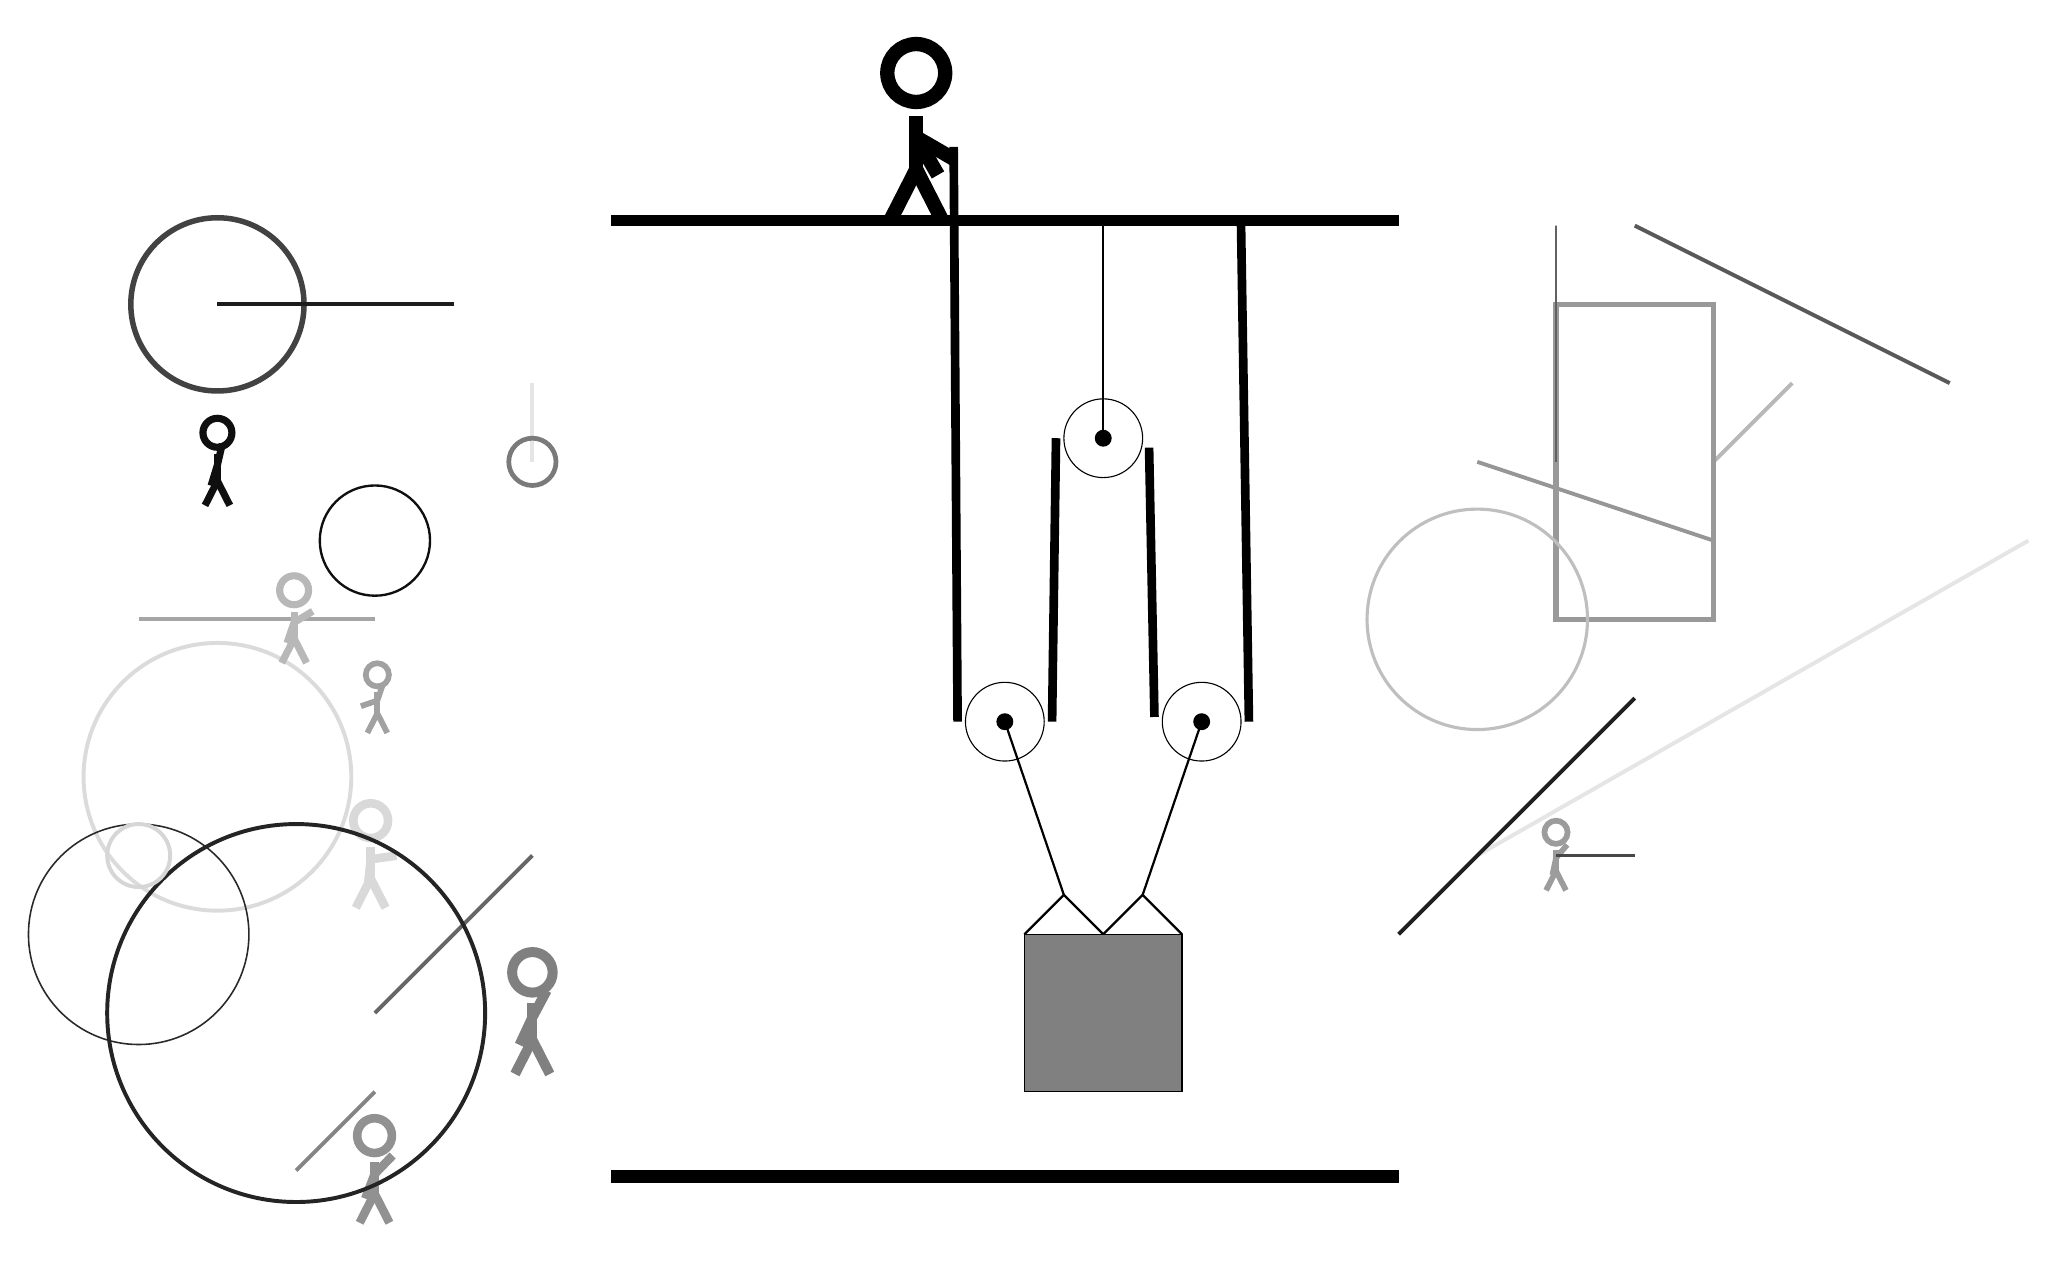
\begin{tikzpicture}
			%%%%% START %%%%%
			
			\draw[fill=black] (-4, 9) rectangle (6, 9.125);
			
			\draw (1, 2.7) circle (0.5);
			\draw[fill=black] (1, 2.7) circle (0.1);
			
			\draw (2.25, 6.3) circle (0.5);
			\draw[fill=black] (2.25, 6.3) circle (0.1);
			\draw[thick] (2.25, 6.3) -- (2.25, 9);
			
			\draw (3.5, 2.7) circle (0.5);
			\draw[fill=black] (3.5, 2.7) circle (0.1);
			
			\draw[thick] (3.5, 2.7) -- (2.75, 0.5);
			\draw[thick] (1, 2.7) -- (1.75, 0.5);
			\draw[thick]  (1.25, 0) -- (1.75, 0.5) -- (2.25, 0);
			\draw[thick]  (2.25, 0) -- (2.75, 0.5) -- (3.25, 0);
			\draw[fill=black!50] (1.25, 0) rectangle (3.25, -2);
			
			\draw[line width=1.1mm] (0.35, 10) --  (0.4, 2.7);
			\centerarc[line width=1.1mm](1, 2.7)(180:360:0.6);
			\draw[line width=1.1mm] (1.6, 2.7) -- (1.65, 6.3);
			\centerarc[line width=1.1mm](2.25, 6.3)(-20:180:0.6);
			\draw[line width=1.1mm](2.832, 6.18) -- (2.9, 2.76);
			\centerarc[line width=1.1mm](3.5, 2.7)(160:360:0.6);
			\draw[line width=1.1mm](4.1, 2.7) -- (4.0, 9);
			
			\draw[line width=0.5mm, color=black!28](11, 7) -- (10, 6);
			
			\draw[line width=0.5mm, color=black!10] (-5, 6) rectangle (-5, 7);
			\draw[line width=0.5mm, color=black!35](-7, 4) -- (-10, 4);
			\draw[line width=0.5mm, color=black!41](10, 5) -- (7, 6);
			
			\draw [line width=0.5mm, color=black!14](-9, 2) circle (1.7);
			\draw [line width=0.7mm, color=black!74](-9, 8) circle (1.1);
			\draw[line width=0.7mm, color=black!40] (8, 4) rectangle (10, 8);
			\draw[line width=0.5mm, color=black!10](7, 1) -- (14, 5);
			\node[line width=0.5mm, color=black!15] at (-7, 1) {\Strichmaxerl[6][84][8]};
			\node[line width=0.4mm, color=black!50] at (-5, -1) {\Strichmaxerl[7][65][62]};
			
			\draw [line width=0.6mm, color=black!52](-5, 6) circle (0.3);
			\node[line width=0.5mm, color=black!43] at (-7, -3) {\Strichmaxerl[6][69][46]};
			\draw[line width=0.5mm, color=black!48](-8, -3) -- (-7, -2);
			
			\node[line width=0.4mm, color=black!39] at (8, 1) {\Strichmaxerl[4][78][50]};
			\draw[line width=0.5mm, color=black!89](-6, 8) -- (-9, 8);
			\node[line width=0.5mm, color=black!28] at (-8, 4) {\Strichmaxerl[5][71][31]};
			
			\draw [line width=0.4mm, color=black!25](7, 4) circle (1.4);
			\node[line width=0.6mm, color=black!37] at (-7, 3) {\Strichmaxerl[4][19][71]};
			\draw[line width=0.5mm, color=black!65](9, 9) -- (13, 7);
			\draw[line width=0.3mm, color=black!72] (8, 1) rectangle (9, 1);
			\draw [line width=0.2mm, color=black!84](-10, 0) circle (1.4);
			
			\draw[line width=0.5mm, color=black!60](-5, 1) -- (-7, -1);
			
			\draw [line width=0.5mm, color=black!86](-8, -1) circle (2.4);
			\draw[line width=0.5mm, color=black!88](6, 0) -- (9, 3);
			\draw[line width=0.2mm, color=black!62] (8, 9) rectangle (8, 6);
			\draw [line width=0.3mm, color=black!94](-7, 5) circle (0.7);
			\node[line width=0.2mm, color=black!94] at (-9, 6) {\Strichmaxerl[5][73][77]};
			\draw [line width=0.5mm, color=black!16](-10, 1) circle (0.4);
			
			\node at (-0.07, 10.2) {\Strichmaxerl[10][120][-30]};
			
			\draw[fill=black] (-4, -3) rectangle (6, -3.15);
			
			%%%%% END %%%%%
		\end{tikzpicture}
	\end{figure}	
\end{document}